\documentclass[a4paper,12pt,bibliography=totoc]{article}
\usepackage[utf8]{inputenc}
\usepackage{graphicx}
\usepackage[hidelinks]{hyperref}
\usepackage{array}
\usepackage{lastpage}
\usepackage{lipsum}
\usepackage{wrapfig}
\usepackage{multirow}
\usepackage{url}
\usepackage{fancyhdr}
\usepackage{titling}
\usepackage{lastpage}
\usepackage[page]{totalcount}
\usepackage[table]{xcolor}
\usepackage{authblk}
\usepackage{csquotes}
\usepackage{epigraph}
\usepackage{movie15}
\usepackage{subcaption}
\usepackage{soul}
\usepackage{pbox}
\usepackage{xcolor}
\usepackage[hmargin=2cm,top=5cm,headheight=75pt,footskip=25pt]{geometry}

\setlength{\parindent}{0.95cm}

\setlength{\epigraphwidth}{0.9\textwidth}


\pagestyle{fancy}

\fancyhf{}
\renewcommand{\headrulewidth}{0pt}
\fancyhead[C]{%
          \setlength{\extrarowheight}{8pt}
          \renewcommand{\arraystretch}{1}
          \begin{tabular}{|m{3.0cm}|m{4.0cm}|m{3.0cm}|m{4.8cm}|}
          \hline
          % start row 1  
		  \multirow{3}{*}{
          	
\includegraphics[width=2.5cm]{logo-dsoft.png}
          } & \multicolumn{3}{m{11.8cm}|}{ 
          	\raggedleft \color[rgb]{.6, 0, 0} \large \fontfamily{ugq}\selectfont DSOFT - Vietnam Joint Stock Company
          } \tabularnewline
          %& 
          %\centering
          %\Huge{TITLE} &
          %\centering
          %\tiny{P\'ag. \thepage\ de \pageref{LastPage}\\
          %Data: 17/05/2013\\
          %Rev. 0}
          \cline{2-4}    
          % start row 2    
          \renewcommand{\arraystretch}{1}     
           & \multicolumn{2}{m{7.0cm}|}{\raggedleft \footnotesize Capstone Project 1 }
          & \raggedleft \scriptsize \url{http://www.d-soft.com.vn}         
          \tabularnewline
          \cline{2-4}    
          % start row 3         
           & \raggedleft \footnotesize Reference: 
           & \raggedleft \footnotesize Revision: 0.1 
           & \raggedleft \scriptsize \url{dsoft@d-soft.com.vn}                  
          \tabularnewline
          \hline        
          \end{tabular}%
}
\renewcommand{\footrulewidth}{0.4pt}
\rfoot{\small Page: {\thepage} of {\getpagerefnumber{LastPage}}}
\lfoot{\small D-Soft ML Training Course}


\fancypagestyle{plain}{%
\renewcommand{\headrulewidth}{0pt}
\fancyhead[C]{%
          \setlength{\extrarowheight}{8pt}
          \renewcommand{\arraystretch}{1}
          \begin{tabular}{|m{3.0cm}|m{4.0cm}|m{3.0cm}|m{4.8cm}|}
          \hline
          % start row 1  
		  \multirow{3}{*}{
          	
\includegraphics[width=2.5cm]{logo-dsoft.png}
          } & \multicolumn{3}{m{11.8cm}|}{ 
          	\raggedleft \color[rgb]{.6, 0, 0} \large \fontfamily{ugq}\selectfont DSOFT - Vietnam Joint Stock Company
          } \tabularnewline
          %& 
          %\centering
          %\Huge{TITLE} &
          %\centering
          %\tiny{P\'ag. \thepage\ de \pageref{LastPage}\\
          %Data: 17/05/2013\\
          %Rev. 0}
          \cline{2-4}    
          % start row 2    
          \renewcommand{\arraystretch}{1}     
           & \multicolumn{2}{m{7.0cm}|}{\raggedleft \footnotesize Capstone Project 1 }
          & \raggedleft \scriptsize \url{http://www.d-soft.com.vn}         
          \tabularnewline
          \cline{2-4}    
          % start row 3         
           & \raggedleft \footnotesize Reference: 
           & \raggedleft \footnotesize Revision: 0.1 
           & \raggedleft \scriptsize \url{dsoft@d-soft.com.vn}                  
          \tabularnewline
          \hline        
          \end{tabular}%
}
}

\setlength\parindent{12pt}



\title{
%
\includegraphics[width=18cm]{img/logo-dsoft.png} \\
%\vspace*{6cm}
\textbf{Age and Gender Classification} \\
\textit{(Specifications)}
}

\author{
Bui Gia Huy\thanks{Artificial Intelligence Department} \thanks{Email: \url{huygb@vietnews24.com}}
}
\date{\textbf{\today}}


%\fancyfoot[C]{%
%          \begin{tabular}{|m{3.0cm}|m{10.0cm}|m{2.5cm}|}
%          \hline
%          \includegraphics[height=1.5cm,width=2.5cm]{logo.png} &
%          \centering
%          \Huge{TITLE} &
%          \centering
%          \tiny{P\'ag. \thepage\ de \pageref{LastPage}\\
%          Data: 17/05/2013\\
%          Rev. 0}\tabularnewline
%          \hline
%          \end{tabular}%
%}
\usepackage{amsmath}
\usepackage{graphicx}
\graphicspath{ {./figs/} }
\begin{document}
%--------------------Title Page
\maketitle
\newpage
%--------------------Change Log Page
\begin{center}
\setlength{\extrarowheight}{5pt}
\begin{tabular}{|m{1cm}|m{4cm}|m{2.5cm}|m{2cm}|m{2.5cm}|m{2cm}|} 
 \hline
 \multicolumn{6}{|m{17cm}|}{\cellcolor{red!25} \Large \textbf{DOCUMENT CHANGE LOG}}
 \\
 \hline
\centering \textbf{Rev.} & \centering \textbf{Description} & \centering \textbf{Author} & \centering \textbf{Date} & \centering \textbf{Approved} & \textbf{Date} \\
 \hline
 0.1 & Draft 1 & Huy G.B & 2019/03/04
 & & \\
 \hline
 &  &  &  & & \\
 \hline
 &  &  &  & & \\
 \hline
 \multicolumn{6}{|m{17cm}|}{\cellcolor{red!25} This document has been based on template TL-SSW-101 Revision 2.0}
 \\
 \hline
\end{tabular}
\end{center}
\newpage
%--------------------ToC Page
\tableofcontents
\newpage
%--------------------Begin Outline
\section{Introduction}
- This \textit{Casptone Project 1} assits for my learning about Machine learning and Deep learning in training course of D-Soft company that Mr. Trung Anh is my supervisor. \\
- Through this project, i want to improve some skills about coding, researching relate to machine learning.\\
- It has a lot of interesting applications about machine learning but in this project i will choose topic \textbf{Age and Gender Classification} because D-Soft company where i am working, has a project relate to this problem.\\
- Basically, my application, which I build, has a website interface that anyone can also access. At that, website allows you submit an image of single people and then it will returns information about age and gender of person inside the picture.\\

\subsection{Purpose}
- Reinforce knownledge about machine learning learned from Coursera \textit{Andrew Ng.}\\
- Build a funny application that apply machine learning to a real world problem.
\subsection{Scope}
- This project in range of D-Soft's training course.\\
- The project focus mainly about: \\
\indent + Build a simple web frontend and backend. \\
\indent + Training a machine learning algorithm.

\newpage
\section{Related Works}
- The system that i build relate to \textbf{classification} problem so it is useful to list some machine leaning algorithm.\\
- In addition to ML algorithms serve for classfy age and gender of a single people, the system is also needed host on a server for demo session. Thus, we will introduce some concepts relate to \textit{Web Application} such as \textit{Frontend} and \textit{Backend}.
\subsection{Classification algorithms}
- It has a lot of machine learning alogrithms relate to classification problem but here, I only introduce some ones that I learned.
\subsubsection{Perceptron}
- In machine learning, the \textbf{perceptron} is an algorithm for \textbf{supervise learning} of \textbf{binary classification}. A binary classfier a function which can decide whether or not an input, represented by a vector of numbers, belongs to some specific class. It a type of \textbf{linear classifier}, i.e. a classification algorithm that makes its predictions based on a linear predictor function combining a set of weights with the feature vector.\\
- In the modern sense, the perceptron is an algorithm for learning a binary classifier called a threshold function: a function that maps its input x (a real-valued vector) to an output value $f(x)$ (a single binary value):\\
$$
f(x) = 
\begin{cases}
1, \indent (w.x + b > 0)\\
0, \indent otherwise
\end{cases}
$$
where \textbf{w} is a vector of real-valued weights, \textbf{w.x} is the dot product $\sum_{i=1}^{m}w_{i}x_{i}$, where \textit{m} is the number of inputs to the perceptron, and \textit{b} is the bias. The bias shifts the decision boundary away from the origin and does not depend on any input value.\\
\\
The value of $f(x)$ (0 or 1) is used to classify x as either a positive or a negative instance, in the case of binary classfication problem. If \textit{b} is negative, then the weighted combination of inputs must produce a postive value greater than $|b|$ in order to push the classfier neuron over the 0 threshold. Spatially, the bias alters the position of the decision boundary. The perceptron learning algorithm does not terminate if the learning set is not linear separable. If the vectors are not linearly separable learning will never reach a point where all vectors are classifed properly. The most famous example of the perceptron's inablity to solve problems with linearly nonseparable vectors is the Boolean exclusive-or problem. The solution spaces of decision boundaries for all binary functions and learning behaviors are studied in the reference.\\
\\
In the context of neural networks, a perceptron is an artifical neuron using the \textit{Heaviside step function} as the activation function. The perceptron algorithm is also termed the \textit{single layer perceptron}, to distinguish it from \textit{multilayer perceptron}, which is a misnomer for a more complicated neural network. As a linear classifier, the single-layer-perceptron is the simplest \textit{feedforward neural network.}\\
\begin{center}
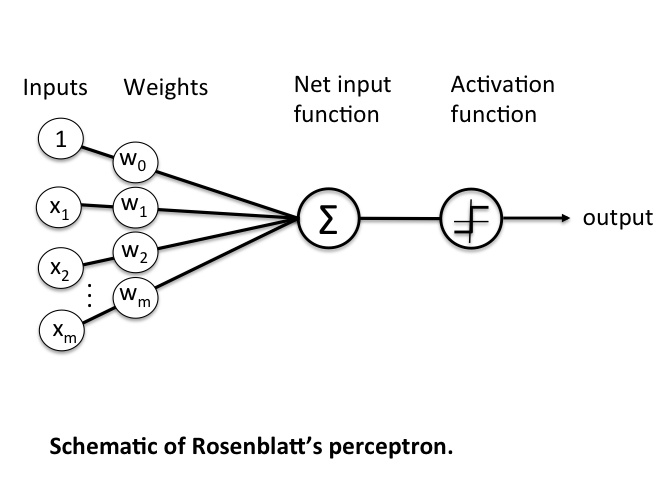
\includegraphics[scale=0.5]{perceptron}\\
\textit{(Source: Sebastian Raschka)}
\end{center}
\subsubsection{Logistic Regression}
- \textbf{Logistic Regression}, also known as \textit{Logit Regression} is a mathematical model used in statics to estimate (guess) the probability of event happens (1) or the event does not happen (0). So given some feature \textbf{x}, it tries to find out whether some event \textbf{y} happens or not. So \textbf{y} can either be 0 or 1. In the case where the event happens, \textbf{y} is given the value 1. If the event does not happen, then \textbf{y} is given the value 0. For example, if \textbf{y} represent whether a sports team wins a match, then \textbf{y} will be 1 if they win the match or \textbf{y} will be 0 if the do not. This is known as \textit{Binomial Logistic Regression}. There is also another form of Logistic Regression which uses multiple values for the variable \textbf{y}. This form of Logistic Regression is known as \textit{Multinomial Logistic Regression}.\\
\\
- Logistic Regession use logistic function to find a model that fits with the data points. The function gives an 'S' shape curve to model to model the data. The curve is restricted betwwen 0 and 1, so it is easy to apply when \textbf{y} is binary. Logistic Regression can then model events better than liner regression, as it shows the probability for \textbf{y} being 1 for a given \textbf{x} value. Logistic Regression is used in statistics and machine learning to predict values of an input from previous test data.\\
\\
Logistic regression is an alternative method to use other than the simpler \textit{Linear Regession}. Linear regression tries to predict the data by finding a linear - straight line - equation to model or predict future data points. logistic regression does not look at the relationship between two variables as a straight line. Instead, Logistic regression uses the logarithm function to find the relationship between the variables and uses test data to find the coefficients. The function can then predict the future results using these coefficients in the logistic equation.\\
\\
Logistic regression uses the concepts of odds ratios to calculate the probability. This is defined as ratio  of the odds of an event happening to ists not happening. For exmaple, the probability of a sports team to win a certain match might be 0.75. The probability for that team to lose would be 1 - 0.75 = 0.25. The odds for that team winning would be 0.75/0.25 = 3. This can be said as the odds of the team winning are 3 to 1.\\
\\
The odds can be defined as:\\
$$
Odds = \frac{P(y = 1|x)}{1 - P(y = 1|x)}
$$
The natural logarithm of the odds ratio is then taken in order to create the logistic equation. The new equation is know as the logit:\\
$$
Logit(P(x)) = \ln \left ( {P(y = 1|x) \over (1 - P(y = 1|x) } \right)
$$
In logistic regression the Logit of the probability is said to be linear with respect to x, so the logit becomes:\\
$$
Logit(P(x)) = a + bx
$$
Using the two equations together then gives the following:\\
$$
{P(y = 1|x) \over 1 - P(y = 1|x)} = e^{a+bx}
$$
This then leads to the probabitly:\\
$$
P(y=1|x) = {e^{a+bx} \over 1 + e^{a+bx}} = {1 \over 1 + e^{-(a + bx)}}
$$
The final equation is the logistic curve for Logistic regression. It models the non-linear relationship between x and y with an 'S-like' curve for the probabilies that y = 1, that event the y occurs. In this example \textbf{a} and \textbf{b} represent the gradients for the logistic function. The logit equation can then be expanded to handle multiple gradients. This gives more freedom with how the logistic curve matches the data. The multiplication of two vectors can then be used to model more gradient values and give the following equation:\\
$$
Logit(P(x)) = w_0x^0 + w_1x^1 + w_2x^2 + ... + w_nx^n = w^Tx
$$
In this equation $w = [w_{0}, w_{1}, ..., w_{n}]$ and represents the n gradients for the equation. The powers of x are given by the vector $x = [1, x, x^{2}, ..., x^{n}]$. These two vectors give the new logit equation with multiple gradients. The logistic equation then can be changed to show this:\\
$$
P(y=1|x) = {1 \over 1 + e^{-(w^Tx)}}
$$
This is then a more genral logistic equation allowing for more gradient values.\\
\begin{center}
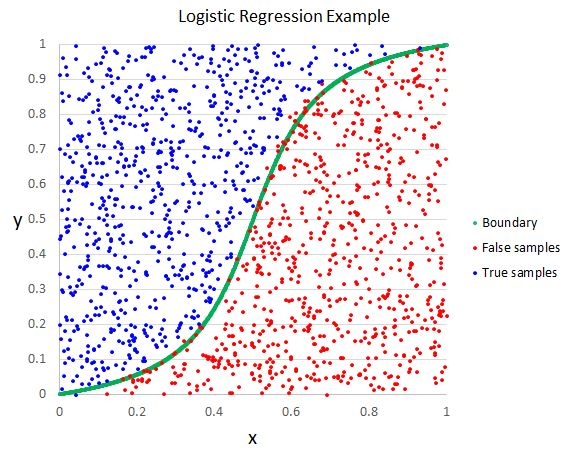
\includegraphics[scale=0.8]{logistic-regression}\\
\textit{(Source: helloacm.com)}
\end{center}
\subsubsection{Artificial Neural Network}
- \textbf{Artificial Neural Networks} (ANN) or \textbf{connectionist systems} are computing systems inspired by the \textit{biological neural networks} that constitute animal brains. The neural network itself is not an algorihm, but rather a framework for many different mahchine learning algorithms to work together and process complex data inputs. Such systems "learn" to perform tasks by considering examples, generally without being programmed with any task-specific rules. For example, in \textit{image recognition}, they might learn to identify images that contains cats by analyzing example images that have been manually labelled as "cat" or "no cat" and using the results to identify cats in other images. They do this without any prior knowledge about cats, for examples, that they have fur, tails, whiskers and cat-like faces. Instead, they automatically gererate identifying characteristics from the learning material that they process.\\
\\
An ANN is based on collection of connected units or nodes called \textit{artificical neurons}, which loosely model the \textit{neurons} in a biological brain. Each connection, like the \textit{sysnapes} in a biological brain, can transmit a signal from one artifical neuron to another. An artifical neuron that receives a signal can process it and then signal additional artifical neurons connected it.\\
\\
In common ANN implementations, the signal at a connection between artifical neurons is \textit{real number}, and the output of each artificial neuron is computed by some non-linear function of the sum of its inputs. The connections between artificial neurons are called 'edges'. Artificial neurons and edges typically have a \textit{weight} that adjust as learning proceeds. The weight increases or decreases the strength of the signal at a connection. Artificial neurons may have a threshold such that the signal is only sent if the aggregate signal crosses that threhold. Typically, artifical neuraons are aggregated into layers. Different layers may perform different kinds of transformations on their inputs. Signals travel from the first layer (the input layer), to the last layer (the output layer), possibly after traversing 
the layer multiple times.\\
\\
The original goal of the ANN approach was to solve problems in the same way that a human brain would. However, over time, attention moved to performing specific tasks, leading to deviations from biology. ANNs have been used on variety of tasks, including \textit{computer vision}, \textit{speech recognition}, \textit{machine translation}, \textit{social network} filteringk, \textit{playing board and video games} and \textit{medical dianosis}.\\
\\
\begin{center}
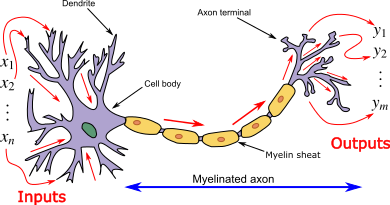
\includegraphics[scale=1]{Neuron3}\\
\textit{Neuron and myelinated axon, with signal flow from inputs at dendrites to outputs at axon terminals.}\\
\textit{(Source: wiki)}
\end{center}
An ANN is an interconnected group of nodes, similar to the vast network of neurons. Here, each node represents an artifical neuron and arrow represent a connection from the output of one artificial neuron to the input of another.\\
\begin{center}
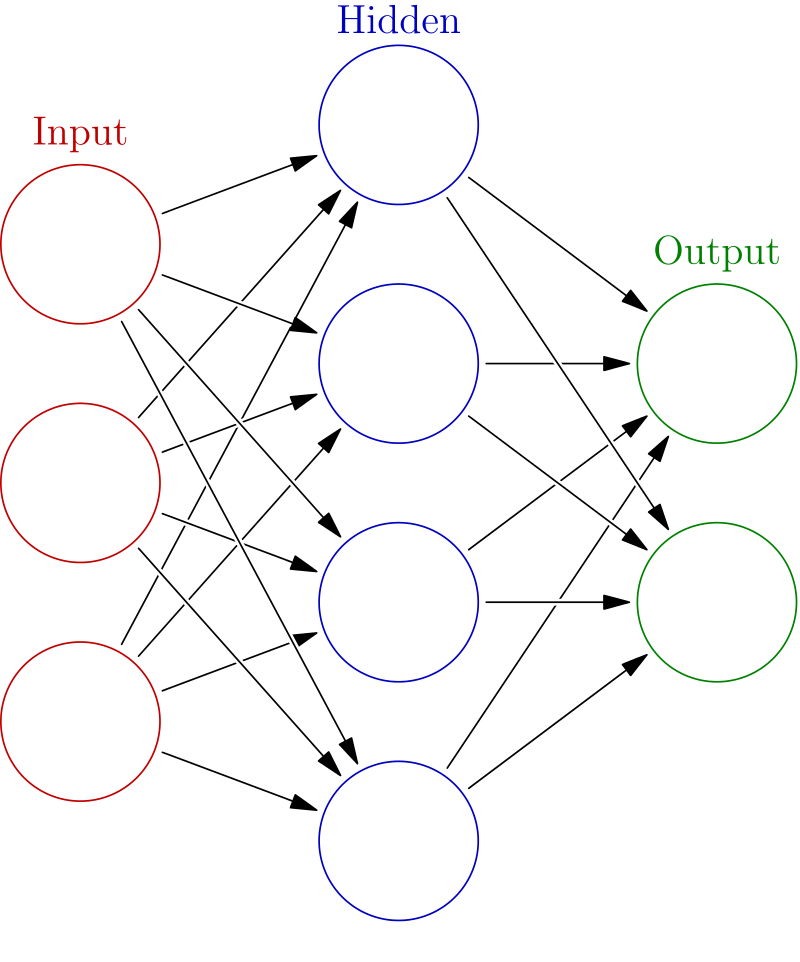
\includegraphics[scale=0.25]{ann}\\
\textit{(Source: wiki)}
\end{center}
\subsection{Web Application}
\subsubsection{Frontend}
\subsubsection{Backend}

\subsection{Example: Dog and Cat Classfication}

\newpage
\section{System Architecure}
\subsection{System Overall}
\subsection{Fronted}
\subsection{Backend}
\subsection{Neural Network}

\newpage
\section{Plan}
\begin{table}[h]
\begin{tabular}{|m{0.3cm}|m{1.0cm}|m{9.7cm}|m{1.6cm}|m{2.4cm}|}
\hline
\multicolumn{5}{|m{17cm}|}{\cellcolor{red!25} \large\textbf{Work Breakdown Structure \& Estimate}} 
\\
\hline
\textbf{\#} & \multicolumn{3}{|m{12.3cm}|}{\textbf{Activities}} & \pbox{2.4cm}{\textbf{~Expected} \\ \textbf{(man-days)}}
\\
\hline
\textbf{1} & \multicolumn{2}{|m{10.7cm}|}{\textbf{Preparation}} & \textbf{1} & 
\\
\hline
& 1.1 & Setup the development environment & & 0.5
\\
\hline
& 1.2 & Search + Pre-processing Dataset & & 0.5
\\
\hline
\textbf{2} & \multicolumn{2}{|m{10.7cm}|}{\textbf{Design and Implement}} & \textbf{3} &
\\
\hline 
& 2.1 & Training + Testing model & & 2
\\
\hline
& 2.2 & Frontend + Backend & & 1
\\
\hline
\multicolumn{2}{|m{1.3cm}|}{} & \multicolumn{2}{m{11.3cm}|}{} &
\\
\hline
\multicolumn{2}{|m{1.3cm}|}{} & \multicolumn{2}{m{11.3cm}|}{\hl{\textbf{Total (man-days)}}} & \hl{\textbf{4}}
\\
\hline

\end{tabular}%
\end{table}

\newpage
\bibliographystyle{unsrt}
\section{References}
1. \url{https://talhassner.github.io/home/publication/2015_CVPR} \\
2. \url{https://talhassner.github.io/home/projects/cnn_agegender/CVPR2015_CNN_AgeGenderEstimation.pdf} \\
3. \url{https://gilscvblog.com/2015/11/19/age-and-gender-classification-using-deep-convolutional-neural-networks/} \\
4. \url{http://dlib.net/} \\
5. \url{https://js.tensorflow.org/} \\

\end{document}